\documentclass[12pt,conference]{IEEEtran}
\usepackage{mathtools}

\usepackage{algorithm}% http://ctan.org/pkg/algorithms
\usepackage{algpseudocode}% http://ctan.org/pkg/algorithmicx

\usepackage{graphicx}
\usepackage{amsmath}

\usepackage{stfloats}
\usepackage{tikz}

\usepackage{amsthm}
\usepackage{amssymb}

\theoremstyle{plain}
\newtheorem{theorem}{Theorem}

\DeclareMathOperator{\atantwo}{atan2}
\graphicspath{ {images/} }

\hyphenation{op-tical net-works semi-conduc-tor}

\begin{document}
\raggedbottom

\title{Fundamentals, Significance and Practicality of Treewidth and Tree Decompositions}

\author{\IEEEauthorblockN{Taylor Cox}
\IEEEauthorblockA{COMP 4060: Graph Theory\\
University of Manitoba\\
Winnipeg, Manitoba\\
Email: coxt3@myumanitoba.ca}}

\maketitle

\begin{abstract}
In 1987, Arnborg proved that it is NP-Complete to determine whether the treewidth of a graph is upper-bounded by some value k. However, Bodlaender proved in 1992 that the treewidth problem is in P in cases where k is fixed. Despite the fact that the treewidth problem is fixed-parameter tractable, the implementation of a general treewidth algorithm has been largely unsuccessful in the graph theory literature. The absence of a comprehensive, practical algorithm for determining the treewidth of a graph leads to the conclusion that fixed-parameter tractibility may not be a sufficiently descriptive characterization of the treewidth problem and related problems.
\end{abstract}

\begin{IEEEkeywords}
Treewidth, Tree Decomposition, Fixed Parameter Tractibility
\end{IEEEkeywords}

\IEEEpeerreviewmaketitle

\section{Introduction}
A key result of Robertson and Seymour's Graph Minor Theory is the notion of treewidth \cite{treewidth-rob-seymour}. Let $G = (V,E)$ be an arbitrary graph. Informally, the treewidth of G $tw(G)$ is an indicator of how similar $G$ is to a tree. Formally, $tw(G)$ is the minimum width across all possible tree decompositions of $G$. A tree decomposition is an organization of $V$ into a collection of bags, where each bag contains one or more vertices and the union of all bags is equal to $V$. The bags are connected such that they form a tree. The width of a tree decomposition is the cardinality of its largest bag minus one. Treewidth-related definitions are further explored in section V.

Many NP-Complete and NP-Hard graph problems are solvable in polynomial time for graphs of bounded treewidth \cite{bodlaender-treewidth-power}. Such problems include Three-Colorability, Max-Clique and Minor Containment. The substantial theoretical significance of the treewidth property has motivated extensive research into approaches for determining the treewidth of a graph. For a general graph $G$ of nonzero genus, it is NP-Complete to determine whether $tw(G) \leq k$ for some $k$. When limited to the planar graphs, is not known whether the treewidth problem is in P or NP \cite{planar-treewidth-unsolved}. Approximation, Heuristic, Dynamic Programming and Fixed-Parameter approaches have all been developed for the purpose of finding the treewidth for general graphs, with varying degrees of success \cite{treewidth-survey}. 

This report evaluates two treewidth algorithms in terms of their programmatic and computational complexity. The first algorithm is Bodlaender's 1992 fixed-paramater treewidth algorithm \cite{bodlaender-1992}, and is ultimately determined to be impractical for usage outside of theoretical computer science. The second algorithm explored is Bodlaender's 2012 dynamic programming algorithm \cite{bodlaender-2012}. A C implementation of this algorithm is benchmarked against the implementation provided in Sage, a standard mathematical software package \cite{sage-original}. Comparative results indicate a need to employ further optimizations in order to decrease the algorithm's runtime. However, the potential for improvement to the algorithm is limited due to its exponential nature. The Sage benchmarks themselves do not run in graphs of more than 100 vertices.

The remainder of this report is structured as follows: Section II captures a formal description of the treewidth problem itself. Sections III and IV describe the background and related literature to the treewidth problem, and outline the motivation for implementing algorithms for treewidth. In sections V through VII, implementations of Bodlaender's 1992 and 2012 algorithms will be described and critically evaluated. Finally, section VIII will deliver the key conclusions of this project, accompanied by possible directions of future work from theoretical and implementation perspectives.

\section{Problem Description}

The treewidth problem is as follows: ``Given a graph G and a positive, nonzero integer k, does G have treewidth at most k?''. The problem is known to be NP-Complete. The treewidth of a graph $tw(G)$ is the minimum width across all possible tree decompositions of G. A \textit{tree decomposition} of a graph is as follows. Let $G=(V,E)$ be an arbitrary graph of more than one vertex. Then the tree decomposition $D = (X,T)$ is a 2-tuple containing $X$ and $T$. $X$ is a collection $X_{1}, X_{2}, ..., X_{m}$ of cardinality $m$. Each subset $X_{i}$ contains some subset of $V$. $T$ is a tree that describes the connections between each subset. The subsets are often referred to as \textit{bags}, and obey the following properties with respect to $G$ and $T$:

\begin{enumerate}
\item $\cup_{X_{i}} = V$
\item Let $X_{i}$ and $X_{j}$ be two distinct members of $X$. If there exists some vertex $u$ such that $u \in X_{i}$ and $u \in X_{j}$, then there exists a path in $T$ from $X_{i}$ to $X_{j}$, such that each $X_{k}$ on the path also includes $u$.
\item Let $u$ and $v$ be two vertices in $G$. If there exists an edge $uv$, then there exists some bag $X_{i}$ that contains both $u$ and $v$.
\end{enumerate}

The \textit{width} of a tree decomposition $w(D)$. is the cardinality of its largest bag, minus one. The treewidth property is therefore always strictly less than the number of vertices in the graph. Subtracting one results in $tw(G)=1$ for trees, which is a more desirable outcome than the treewidth of a tree being two. It is evident from the definition prodivded that multiple tree decompositions are possible for most graphs. However, some graphs induce only one tree decomposition. Since the treewidth of a graph is its minimum possible tree decomposition width, there exist some graphs that have only one possible treewidth.

\begin{theorem}
  $tw(K_{n}) = n-1$
\end{theorem}

\textit{Proof:} Induction is used on $n$. 

Base case: $n=3$. Let $G=K_{n}$ and $D=(X,T)$ be the tree decomposition of $G$. Assume $tw(G) < n-1$. Then each bag in $X$ covers exactly two vertices (there are two such bags and they must be connected). Therefore, there exists an edge $uv$ such that neither bag in $X$ contains both $u$ and $v$. Let $Y$ be a new bag consisting of $u,v$. Since $uv$ is the only edge not present in the decomposition, $Y$ will be connected in $T$ to both existing bags in $X$, one of which containing $u$ and the other containing $v$. However, the two existing bags in the decomposition are already connected. Therefore, connecting $Y$ to both bags induces a cycle in $T$. Contradiction. $uv$ must be introduced to the decomposition by appending $v$ into the bag containing $u$. The result is a bag containing $n$ vertices. Since a bag in $X$ contains $n$ vertices, no other bags are needed. The treewidth of $K_{n}$ for $n=3$ is therefore 2. 

Induction case: Assume $tw(K_{n-1}) = n-1$. Let $D=(X,T)$ be the tree decomposition of $K_{n-1}$. $K_{n}$ is generated from $K_{n-1}$ by introducing a vertex $u$ and connecting it to all vertices. Partition the endpoints of edges in $K_{n}$ containing $u$ into two or more bags Each new bag will also contain $u$, and is connected to the original bag in $D$. Since each bag contains $u$, the bags are also connected to eachother in a path. This induces a cycle in $T$. Contradiction. The only way to introduce $u$ is by composing a single bag containing the endpoints of all edges departing from $u$. The result is a single bag containing all $n$ vertices, which must have treewidth $n-1$. $\square$
\\
\\
A tree decomposition is considered minimal when none of its bags may be reduced in size without affecting the decomposition's correctness. Since $tw(G)$ is the minimum decomposition width across all possible tree decompositions of G, $tw(G)$ is equal to the width of the \textit{minimal} tree decomposition of G. Figure (1) shows the tree decomposition of a graph on 7 vertices, accompanied by a minimal tree decomposition. The treewidth of the graph shown is 3. Let $D_{min}$ be the minimal decomposition of $G$. Since $tw(G) = w(D_{min})$, knowing the treewidth of $G$ is equivalent to knowing its minimal tree decomposition. Since non-minimal tree decompositions are equally or less powerful than minimal tree decompositions, only minimal decompositions will be considered for the remainder of this report.

\begin{theorem}
  Let $C$ be the max clique in $G$. Then $tw(G) \geq |C|-1$.
\end{theorem}

\textit{Proof:} Let $D=(X,T)$ be the (minimal) tree decomposition of $G$. By (1) and (2) of the tree decomposition definition, the endpoints of each edge in $C$ are included in some $X_{i}$, and the bags containing each vertex in $C$ are connected. Since an edge exists between every vertex pair in $C$, the bags formed by $C$ must be interconnected. Interconnected bags form a cycle. Contradiction. The vertices of $C$ are part of or form a single bag $Y$. If $Y$ is the largest bag and $Y=C$, $tw(G)=|C|-1$. Otherwise, $tw(G) > |C|-1$. $\square$
\\
\\
The treewidth problem is NP-Complete, and the minimal tree decomposition problem is NP-Hard. Even to the trained eye, instances of either problem involving more than a small number of vertices generally require computer aid. Since treewidth is derived from tree decompositions, the treewidth problem may only be solved by finding a minimal tree decomposition. The continued research efforts in the treewidth problem are motivated by the substantial benefits of the treewidth property. The background and motivations behind solving the treewidth problem are now discussed.

\begin{figure}[H]
\begin{center}
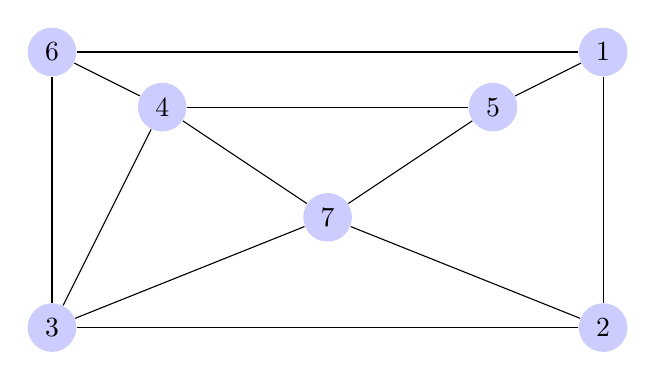
\begin{tikzpicture}
  [scale=.7,auto=right,every node/.style={circle,fill=blue!20}]
  \node (n6) at (5,10) {6};
  \node (n4) at (7,9)  {4};
  \node (n5) at (13,9)  {5};
  \node (n1) at (15,10) {1};
  \node (n2) at (15,5)  {2};
  \node (n3) at (5,5)  {3};
  \node (n7) at (10,7)  {7};

  \foreach \from/\to in {n1/n2,n6/n1,n6/n3,n7/n2,n7/n3,n7/n4,n7/n5,n6/n4,n4/n5,n5/n1,n2/n3,n3/n4}
    \draw (\from) -- (\to);
\end{tikzpicture}
\end{center}
\end{figure}

\begin{figure}[H]
\begin{center}
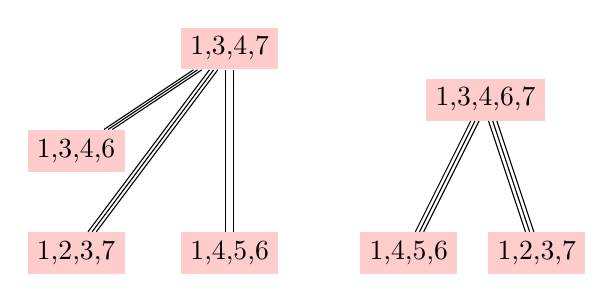
\begin{tikzpicture}
  [scale=.65,auto=right,every node/.style={fill=red!20}]
  \node (d1) at (9, 13) {1,3,4,6,7};
  \node (d2) at (7.5, 10) {1,4,5,6};
  \node (d3) at (10, 10) {1,2,3,7};

  \foreach \from/\to in {d1/d2,d1/d3}
    \draw[transform canvas={xshift=-1.5pt}] (\from) -- (\to);

  \foreach \from/\to in {d1/d2,d1/d3}
    \draw[transform canvas={xshift=1.5pt}] (\from) -- (\to);

  \foreach \from/\to in {d1/d2,d1/d3}
    \draw (\from) -- (\to);

  \node (d5) at (4, 14) {1,3,4,7};
  \node (d6) at (4, 10) {1,4,5,6};
  \node (d7) at (1, 10) {1,2,3,7};
  \node (d8) at (1, 12) {1,3,4,6};

  \foreach \from/\to in {d5/d6,d5/d7,d5/d8}
    \draw[transform canvas={xshift=-1.5pt}] (\from) -- (\to);

  \foreach \from/\to in {d5/d6,d5/d7,d5/d8}
    \draw[transform canvas={xshift=1.5pt}] (\from) -- (\to);

  \foreach \from/\to in {d5/d7,d5/d8}
    \draw (\from) -- (\to);

\end{tikzpicture}

\end{center}
\caption{Two tree decompositions of a graph. One is minimal and the other is not. The graph has treewidth 3.}
\end{figure}

\section{Background}

Treewidth and tree decompositions have been thoroughly explored in the literature. Research perspectives include range from the purely theoretical to the purely practical points of view. The first recorded examination of the treewidth property is from Bertelé et al in 1972 \cite{treewidth-original}. Treewidth was originally referred to as graph \textit{dimension}, and was known to be a valuable property with respect to the solvability of NP-hard problems. The treewidth literature is primarily categorized into works developing methods for determining treewidth, and works exploring the power of the treewidth property. The remainder of this section is divided the same way.

\subsection{Determining Treewidth}

After initial investigation by Bertelé, the treewidth property remained unexplored for some time. In 1984, Robertson and Seymour gave a re-examination of treewidth as part of Graph Minor Theory \cite{treewidth-rob-seymour}. While Robertson and Seymour had shown the theoretical and algorithmic significane of treewidth, no algorithms yet existed to determine $tw(G)$. By 1987, Arnborg had proven that the treewidth problem is NP-Complete \cite{arnborg-np-complete}. However, Bodlaender gave an algorithm in 1992 to determine a fixed-parameter variant of the treewidth problem \cite{bodlaender-1992}. Bodlaender's algorithm answered the following question: ``given a graph G and a \textit{fixed constant} k, does G have treewidth k or less?''. The algorithm proved that the treewidth problem is fixed-parameter tractable. Bodlaender was able to prove that when k is held fixed (and thus is not captured in the O(*) measurement of the algorithm), the algorithm runs in O(n) against the size of the graph. However, the algorithm is known to have a recursive depth of up to $n^{8}$ and depends on a constant as large as $k^{k^{3}}$ \cite{bodlaender-problems}. Therefore, Bodlaender's algorithm is generally considered impractical for implementation \cite{fellows-on-bodlaender}. 

Other alternatives in the literature have been explored for determining $tw(G)$. These alternatives focus on heuristics for treewidth bounding. Many modern heuristics for treewidth rely on the notion of a \textit{perfect elimination ordering}. For $G=(V,E)$, A perfect elimination ordering is an ordering $\pi$ of $V$ where the $i$th vertex of $\pi$ is simplical in the subgraph formed by all vertices from $i$ to $n$. A vertex is simplical if its neighbours induce a clique. Algorithms for generating perfect elimination orderings also serve as heuristics for treewidth upper bounding. 

One heuristic based on simplical vertices and eliminiation orderings is the minimum degree heuristic \cite{min-degree-upper-bound}. In this heuristic, choose a vertex $v$ of minimum degree, introduce edges such that $v$ is simplical. Let the new graph be $G'$. Build a tree decomposition in $G'$ containing some bag $Y$ that covers each neighbour of $v$ (by theorem 2, every clique in $G$ forms a bag in $X$). A new bag - one that contains $v$ and its neighbours - is attached to $Y$. This gives a tree decomposition in $G$. This heuristic may not produce a minimal tree decomposition, but it will give an upper bound for tree width.

The algorithmic focus of this report is on exact algorithms for treewidth. The standard algorithm for determining treewidth is developed by Bodlaender, in 2012 \cite{bodlaender-2012}. The algorithm given uses dynamic programming, and functions similar to the Held-Karp Travelling Salesman Problem dynamic programming algorithm. The algorithm begins with an empty treewidth of infinite weight, and tightens the bound on the treewidth until a minimal decomposition is found. The algorithm takes advantage of the minimax problem that arises in treewidth computation. The algorithm uses that fact treewidth is the \textit{maximum} cardinality of the \textit{minimum} tree decomposition to develop a principle of optimality as needed for a dynamic programming algorithm. The algorithm relies on the max clique of $G$ as a stopping condition, since the $tw(G)$ cannot be exceeded by the cardinality of the max clique. Bodlaender's 2012 dynamic programming algorithm produces exact values for treewidth, but runs in O($2^{n}$) time.

Many algorithms exist to determine or approximate the treewidth of the graph. Since the treewidth problem is NP-Complete and the tree decomposition is NP-Hard, much work has been accomplished to find appropriate limitations to the treewidth problem. These problems include fixed parameter algorithms, heuristics, and bounding approaches. The key algorithms for treewidth are Bodlaender's 1992 and 2012 algorithms. Bodlaender's 1992 algorithm gives a general approach for solving the treewidth problem, but is not practical for implementation. In contrast, Bodlaender's 2012 algorithm is appropriate for implementation, but carries and exceptionally slow runtime. Section V covers both of Bodlaender's algorithms in further detail.

\subsection{Treewidth Significance}

Robertson and Seymour had used treewidth as part of their efforts to prove Wagner's Conjecture. They first determined that planar graphs of bounded treewidth formed a well-quasi-ordering: for any planar obstruction, the family of planar graphs characterized by that obstruction have a treewidth bounded by the size of the obstruction \cite{seymour-stack-overflow}. The usage of treewidth bounding as part of minor closed-well-quasi ordering for general graphs would constitute the next step of Robertson and Seymour's work.

\section{Motivation}

\section{Solution Techniques}

\section{Experimental Setup}

\section{Experimental Results}

\section{Conclusions and Future Work}

\begin{thebibliography}{1}
\bibitem{treewidth-rob-seymour}
\bibitem{bodlaender-treewidth-power}
\bibitem{planar-treewidth-unsolved}
\bibitem{treewidth-survey}
\bibitem{bodlaender-1992}
\bibitem{bodlaender-2012}
\bibitem{sage-original}
\bibitem{treewidth-original}
\bibitem{arnborg-np-complete}
\bibitem{bodlaender-problems}
\bibitem{fellows-on-bodlaender}
\bibitem{min-degree-upper-bound}
\bibitem{seymour-stack-overflow}
\end{thebibliography}

\end{document}
